\chapter{LITERATURE REVIEW}
\label{chapter:literature_review}

\par
The initial phase of the thesis was getting familiar with concept of \acrshort{mbt}, analyzing previously done or currently ongoing researches and case studies related to \acrshort{mbt} and choosing the right tool which conformed with our requirements through literature review. Within this phase 16 research papers, 1 master's thesis and 1 patent description were read completely, analyzed and documented, not to mention tool descriptions as well as other papers which were discarded after reading the abstract. It also included time during which multiple \acrshort{mbt} tools were configured and tried out for choosing one for applying it for \acrshort{bsc}. Overall, 2 complete months were spent on the literature review, results and highlights of which can be read in sections below.

\section{Modeling Paradigms}

\par
As the extensive research has been done for already couple of decades related to usage of modeling in software development, this resulted in multiple modeling paradigms available today. According to survey on \acrshort{mbt} approaches done in 2007 \cite{Survey} reader can observe list of most popular modeling notations in the table \ref{tab:Usage_Survey}. 

\begin{table}[]
    \centering
    \begin{tabular}{|c|c|}
        \hline
        Modeling Notations & Usage Amounts \\
        \hline
        Statechart Diagram & 27 \\
        \hline
        Class Diagram & 19 \\
        \hline
        Sequence Diagram & 19 \\
        \hline
        Use Case Diagram & 11 \\
        \hline
        OCL & 11 \\
        \hline
        (Extended) Finite State Machine & 10 \\
        \hline
        Activity Diagram & 9 \\
        \hline
        Collaboration Diagram & 8 \\
        \hline
        Object Diagram & 7 \\
        \hline
        Graph & 7 \\
        \hline
        Z Specification & 4 \\
        \hline
    \end{tabular}
    \caption{Usage of \acrshort{mbt} notations \cite{Survey}}
    \label{tab:Usage_Survey}
\end{table}

Multiple modeling paradigms are perfectly described and analyzed by Utting et. al. in a taxonomy of model-based testing approaches \cite{Pretschner_Taxonomy}. According to our business needs two of them, State-based notations and Transition-based notations are useful and worth describing in more details in following subsections. Also we cannot omit flowcharts which have been proven to be very useful in modeling processes, systems and programs. 

\subsection{Flowchart}
\par
Flowchart \cite{Flowchart} is extremely useful for modeling workflow or process. Typical flowchart consists of activity and decision points and flowlines which is used for interconnecting them. Other potential building blocks of flowchart are terminal responsible for depicting beginning and ending of the flow, Input/Output responsible for entering data and displaying results, annotations for displaying additional information about steps and predefined processes which are shown in flowchart but defined somewhere else. Different types of flowcharts can be encountered such as document, data, system and program flowcharts. They show controls over document-flow, data-flow, system's physical and resource level and program respectively.

\subsection{State-based Notations}
\par
Internal state of the system is modeled as a set of variables which are edited by operations. Usually, each operation contains pre and post condition which verifies updates the state.\cite{Pretschner_Taxonomy} State-based modeling is supported by multiple notations such as Z, Spec\#, \acrshort{ocl} and others. Applying state-based modeling paradigm requires knowledge of at least one of these modeling notations, which makes it more difficult to apply it within company, without significant changes such as teaching responsible for modeling people one of these notation or employing new people who are already proficient with it. 

\subsection{Transition-based Notations}
\par
Transition-based notations are used for describing transitions between different states of application. Typical representation of it would be \acrshort{fsm}, in which, nodes represent the state of application and edges refer to actions which are required for transition from one state to another. \acrshort{fsm} can be enhanced with data variables which will result in \acrshort{efsm}, as well as with operational profiles which would make Markov Chain out of this \acrshort{fsm}. There are other ways as well to make \acrshort{fsm} more expressive, such as hierarchies of machines and parallelism between machines\cite{Pretschner_Taxonomy}.

\section{Tool Review}
During the literature review we encountered significant amount of case-studies with different tools applied for \acrshort{mbt} which are: USE, Alloy Analyzer, ZLive, ProZ, Spec Exlorer, NModel, T2D4WSC, Graphwalker, TVT, MobiGUITAR and TestCast. CA Agile Requirement Designer cannot be omitted as well, even though it was not found through case-studies. After analysis of all of them, most suitable for us tools are described in details below.

\subsection{Spec Explorer}
\par
Spec Explorer \cite{SpecExplorer_Description} is a \acrshort{mbt} tool which has been developed by Microsoft Research between 2004 and 2010. It has been used within Microsoft for testing on a daily basis. Spec Explorer is an Add-On to Microsoft Visual Studio \acrshort{ide}, but now we can assume that it has been deprecated due to non-compatibility with the newer versions of Visual Studio \acrshort{ide} released after 2012.
\par
Models in Spec Explorer are written as a program code. For writing models all .NET language are supported, such as C\#. Written models contain a set of rules which interact with a defined state. Cord is a scripting language, which is used for combining the model programs. This provides a description to the test generation algorithms in which ways a model program can be explored. Model program together with Cord scripts generate a behavioral model of \acrlong{aut}.

\par
Spec Explorer applies state-based modeling paradigm and the created behavioral models are represented in a form of \acrshort{fsm}. It applies different coverage criteria for test generation, such as data coverage of parameter values, coverage of state space or coverage of all transitions through model. Test generation could be off-line as well as be applied together with the execution on-line.

\par
Spec Explorer also has a model viewer module in which the user can see the visual representation of created behavioral model. A representation of the same is shown in the figure \ref{Fig:Model_View_In_SpecExplorer}.

\begin{figure} [htbp!]
	\centering
					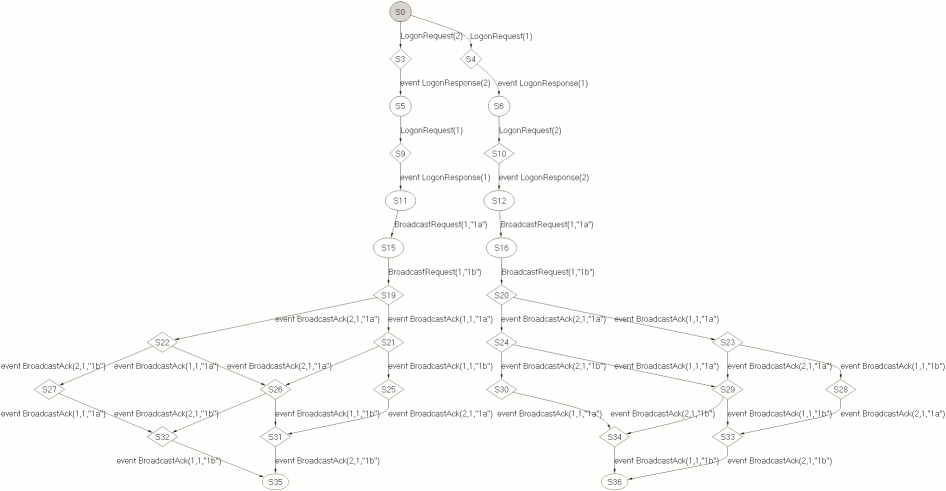
\includegraphics[width=1\textwidth]{figures/Model_View_In_SpecExplorer.png}
					\caption{\label{Fig:Model_View_In_SpecExplorer} Visual Representation of Model in Spec Explorer \cite{SpecExplorer_ModelView}}
\end{figure}

\par
When a \acrshort{fsm} is created and it has extensively big or even infinite state space, a technique called Slicing is used for generation of smaller subsets of the full behavior models which are more suitable for testing.

\par
One of the examples for usage of Spec Explorer in practice was provided by Jose L. Silva et. al. \cite{Silva_SpecExplorer} where they applied it together with ConcurTaskTrees. They created task models using ConcurTaskTrees notation
and used a tool TERESA for generating \acrshort{fsm} from it. For creating the Spec\# model, generated \acrshort{fsm} is given as an input to a tool called TOM (Task to Oracle Mapping tool) which was developed in scope of that research. The last step was the generation of tests from the Spec\# models using Spec Explorer and mapping the generated tests to a test driver which would then execute test against the \acrshort{aut}.

\subsection{NModel}
\par
NModel \cite{NModel_Description} \cite{NModel_Description2} is a modeling framework based on the usage experiences of Spec Explorer. Unlike the Spec Explorer, which uses separate compiler for compiling Spec\# models, NModel uses the standard .NET v2.0 compiler. Modeling with NModel requires coding knowledge since models are required to be implemented using C\#.

\par
Based on the obtained model, NModel generates a \acrshort{fsm} or an \acrshort{efsm} which can later be traversed with different coverage criteria passed to modules responsible for the test generation.

\par
NModel is made up of multiple artifacts. The NModel library consists of attributes and data types for writing models. The Model Program Viewer (mpv) and the Model Program to Dot (mp2dot) are modules responsible for visualization and analysis of the created model.The Model Program Viewer can be visualized in the figure below. The Offline Test Generator (otg) provides an opportunity to generate the test suite off-line. The Conformance Tester (ct) module can be used in both ways, off-line as well as on-line \acrshort{mbt}.

\begin{figure} [htbp!]
	\centering
					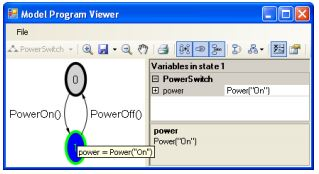
\includegraphics[width=0.5\textwidth]{figures/NModel_mpv.JPG}
					\caption{\label{Fig:NModel_mpv} Model Program Viewer of NModel}
\end{figure}


\par
We came across the usage of NModel a couple of times during the literature review. In one of them Chinnapongse et. al. \cite{Chinnapongse_NModel} used NModel for testing \acrshort{gui} of The Armed Forces Health Longitudinal Tracking Application–Mobile (AHLTA-Mobile). The application is based on a Windows Phone platform containing multiple modules. In the scope of their research, the Military Acute Concussion Evaluation (MACE) module consisting of 8 different GUI Screens was tested. They began with creating the mental model of the application first, which was later coded in C\#. The resulting artifact was an \acrshort{efsm} that was used to generate tests off-line. The last part was executing the generated tests against the MACE module.
\par
Another user of NModel was Gabriel Kolawole \cite{Kolawole_NModel} who tested \acrshort{gui} and functionality of the Moodle Mobile Application in his master thesis.

\subsection{MobiGUITAR}
\par
MobiGUITAR \cite{MobiGUITAR} was introduced with a collaboration of researchers from the University of Naples Federico II and the University of Maryland. Their previous project, GUI ripping \cite{GUIripping}, was created for desktop applications and was based on \acrshort{efg}, but as mobile applications are very state sensitive, they decided to change their approach and made a MobiGUITAR based on a \acrshort{fsm}. Currently MobiGUITAR is limited to the android platform.

\par
The testing process with MobiGUITAR is divided into three phases: ripping, generating and executing. Ripping dynamically explores the application and creates a \acrshort{fsm} with the application states and events. An example of a generated \acrshort{fsm} can be seen in the figure \ref{Fig:MobiGuitar}.

\begin{figure} [htbp!]
	\centering
					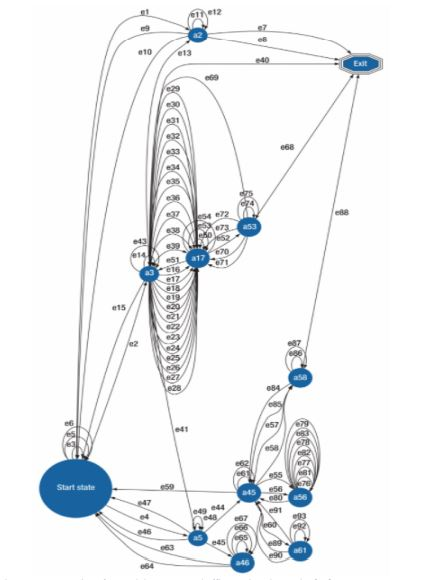
\includegraphics[width=0.5\textwidth]{figures/mobiguitar.JPG}
					\caption{\label{Fig:MobiGuitar} The abstract state machine for AardDict\cite{MobiGUITAR}}
\end{figure}

During the generation phase a \acrshort{fsm} is created along with a coverage criteria, such as pair-wise edge coverage to generate the test cases. This means that all the pairs of the adjacent edges are required to be taken together.
The execution phase applies a JUnit framework for testing the \acrshort{aut} and returning the results to a tester. Basically, with these 3 phases together the MobiGUITAR automates not only test generation and execution, but also the entire modeling process itself, which gives it an advantage over other \acrshort{mbt} tools.

\par
Inability of functional testing is the main disadvantage which MobiGUITAR has. It is mentioned in \cite{MobiGUITAR} that, tester can enhance the JUnit tests with assertions for detecting functional errors, but that will not be easy task, because assertion of states might strongly depend with which event this state is reached. Besides that, after firing same event from same state, depending on background variables landing state might be different. For applications such as \acrshort{bsc}, verifying that functional part works as designed has the highest priority while testing that \acrshort{gui} is displayed correctly has a bit lower priority. MobiGUITAR would be very useful for example for verification of \acrshort{gui} correctness, or verification that there are no crashes and unhandled exceptions after transitions from one state to another. But in our case, that is definately not enough.

\subsection{Graphwalker}
\par
Graphwalker \cite{Graphwalker_Description} is an open-source tool for \acrshort{mbt}. It was originaly developed using the Java programming language, but now the Python implementation is also made available. It was created by the developers at Spotify \cite{Spotify} and is maintained by them through the open source community. Graphwalker takes the \acrshort{fsm} or the \acrshort{efsm} created with a set of predefined rules as an input and traverses it with a given coverage criterion.
The example input model can be observed in the figure below \ref{Fig:Graphwalker_model_example}.

\begin{figure} [htbp!]
	\centering
					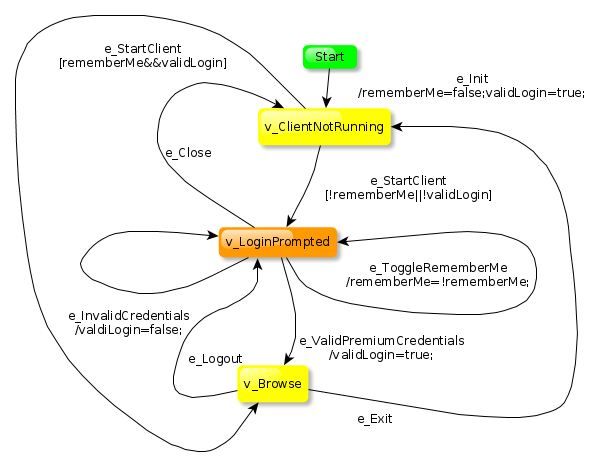
\includegraphics[width=0.8\textwidth]{figures/Graphwalker_model_example.png}
					\caption{\label{Fig:Graphwalker_model_example} Graphwalker input model example \cite{Graphwalker_Login_Example}}
\end{figure}

\par
The modeling part currently needs to be done completely independent from the Graphwalker software. yEd Graph Editor \cite{yEd} is the tool currently suggested for creating models for Graphwalker and the team is working on producing an internal modeling tool for the next release. Graphwalker supports off-line test generation, for which a basic knowledge of the command line interface is required by the user. The on-line test generation and execution is performed with tests written in Java or Python. 

\par
Graphwalker allows splitting models with shared steps. For example, when a model is huge and not readable, or if the user wants to separate a model into different functional parts of the system, he/she can annotate the vertex with Shared keyword which will let Graphwalker know that while traversing it can find similar state in other models as well.

\par
The biggest advantage of the Graphwalker among the discussed modeling tools is that, very little new skills are required by the testers in a company to create the models for the Graphwalker and also very minimal effort is required by them to generate tests off-line from the created model. If the test execution automation is not available, user can execute generated tests manually against the \acrshort{aut}, which is also the current the plan of this thesis.

\par
A couple of case-studies were encountered relating to the Graphwalker during the literature review. One of which described the application of \acrshort{mbt} using the Graphwalker in NASA's Goddard Mission Service Evolution Center (GMSEC) \cite{GMSEC}. \acrshort{mbt} approach was applied to the software bus project which was based on a pub-sub architecture. Different applications could be connected using middle-ware wrappers and publish and subscribe messages related to the subjects. As a result new bugs were found, which were not detected by the existing testing process. The paper contains a comparison between the effort and the results of using both \acrshort{fsm} and \acrshort{efsm}. It shows what are the capabilities that were lacking from the \acrshort{fsm} such as not being able to embed assertions in states which was leading to the inability to test different functionality and how \acrshort{efsm} enabled to test them. Use of legacy test cases were also quite useful for modeling the \acrshort{aut}, because the specification and the documentation were ambiguous and describing functionality that was not implemented at all and would result in a wastage of the modeling time.

\subsection{USE}
\par
USE (\acrshort{uml}-based Specification Environment) \cite{USE_definition} is a tool based on \acrshort{uml} modeling language enhanced with \acrshort{ocl} constraints. Its purpose is to assist analysts, designers and developers in executing \acrshort{uml} models and checking \acrshort{ocl} constraints. System models, invariants,  pre an post conditions can be specified in a textual form. Models are defined in a .use file and generation of its instances is orchestrated by .assl file. The file with .ins extension contains extra optional invariants. Generation of snapshots is done by user through editing .assl file. Figure \ref{Fig:USE_test_generation} shows structure of .assl file.

\begin{figure} [htbp!]
	\centering
					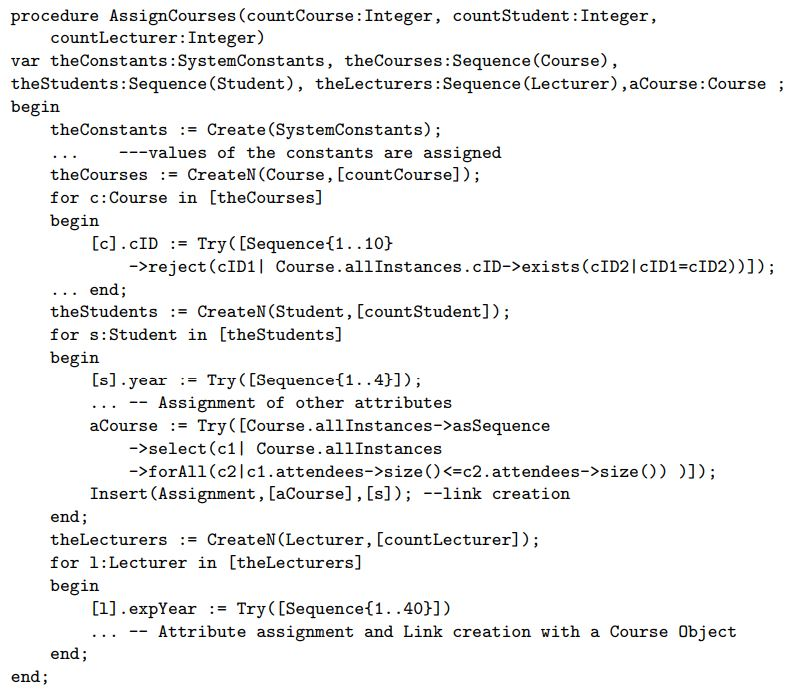
\includegraphics[width=0.8\textwidth]{figures/USE_test_generation.JPG}
					\caption{\label{Fig:USE_test_generation} Example of .assl file \cite{USE_Alloy_Z_comparison}}
\end{figure}

\par
One usage of USE tools can be observed in \cite{USE_Alloy_Z_comparison} where it is compared to other tools such as Alloy Analyzer, ProZ and Zlive in order to detect abilities and weaknesses of tools for different modelling languages. For this purpose, they conducted simple experiment with Course Assignment System, which was written in 3 different modeling languages, \acrshort{uml} enahnced with \acrshort{ocl}, Alloy and Z. Then they used above mentioned tools respectively and compared the results.

\subsection{Agile Requirements Designer from CA Technologies}
\par
Agile Requirements Designer if a \acrshort{mbt} commercial tool developed by CA Technologies\cite{Agile_Requirement_Designer_desciption}. Models are represented in form of flowcharts. It can be used for off-line as well as on-line execution. The example model could be observed in the figure \ref{Fig:AgileRequirementDesigner_Charts}. It supports multiple coverage criteria such coverage of all paths, all edges, all nodes and pairwise edge coverage.

\begin{figure} [htbp!]
	\centering
					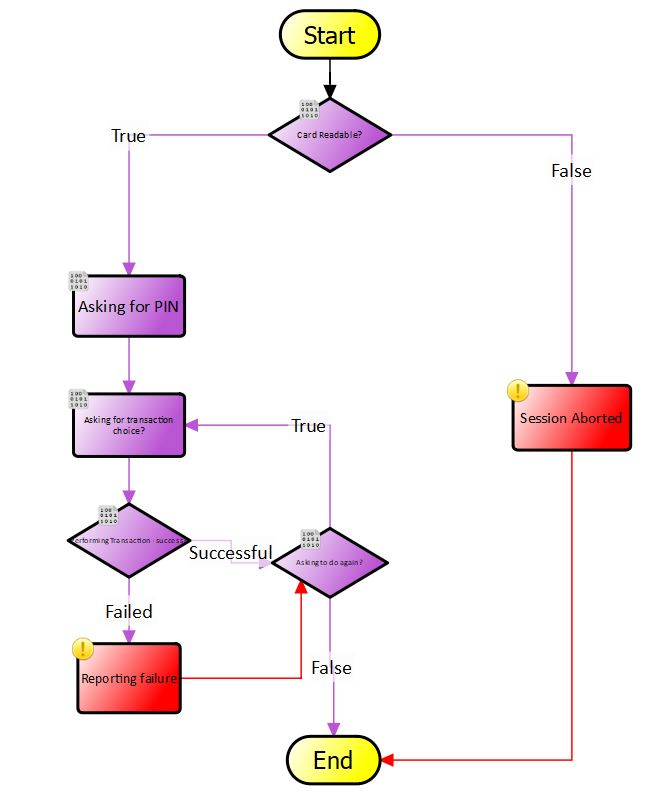
\includegraphics[width=0.8\textwidth]{figures/AgileRequirementDesigner_Charts.JPG}
					\caption{\label{Fig:AgileRequirementDesigner_Charts} Model in Agile Requirement Designer}
\end{figure}

\par
CA Technologies provides more tools for testing such as CA Test Data Manager which, together with Agile Requirement Designer broadens the opportunities for providing high coverage during software testing. Agile Requirement Designer has integration interfaces to popular issue tracker software such as Microsoft TFS, Atlassian Jira and others. These interfaces give opportunity to directly add or alter generated test cases from models to an issue tracker software used by company. Agile Requirement Designer also provides interfaces for connection to popular test execution automation engines, such as Ranorex and others.

\par
To sum up, Agile Requirement Designer gives opportunity to integrate \acrshort{mbt} into the company with less changes required for current testing process. It would be our first choice, but unfortunately, we did not get answer to our request for using it in scope of this thesis.

\section{Justification of Decision}

\par
Basically, all tools reviewed in previous section were suitable for applying off-line \acrshort{mbt} for \acrshort{bsc} except MobiGUITAR which supports only android platform. So, Prioritization of the rest of the tools were based on the requirements given from company that the chosen tool should be usable among all quality engineers in company. USE required adoption of \acrshort{uml} as well as language for writing generation criteria in .assl file, because of this it got the lowest priority. NModel and Spec Explorer required knowledge of programming languages and programming concepts which reduced their priority in our list as well. Among remaining two tools, CA Agile Requirement Designer had higher priority due to its connection interfaces to many other already used technologies in Brainloop, which was making it easier to integrate \acrshort{mbt} into the current testing process, but unfortunately we were not responded for the request of using it during our thesis. As a result, choice was made in advantage of Graphwalker. Table \ref{tab:Prioritized_Tools} summarizes the prioritization of underlying tools.

\begin{table}[]
    \centering
    \begin{tabular}{|l|l|p{8cm}|}
        \hline
        Priority & Tool & Reasons \\
        \hline
        1 & Graphwalker & Requires no programming knowledge for applying off-line \acrshort{mbt} \\
        \hline
        2 & CA Agile Requirement Designer & Easily integratable into Brainloops current testing process. Request for usage was not responded \\
        \hline
        3 & NModel & Requires programming knowledge \\
        \hline
        4 & Spec Explorer & Requires programming knowledge, Product is not maintained any more \\
        \hline
        5 & USE & Requires adoption of new languages for modeling and test generation\\
        \hline
        6 & MobiGUITAR & Supports only android platform \\
        \hline
    \end{tabular}
    \caption{Prioritized Tools}
    \label{tab:Prioritized_Tools}
\end{table}